%%%%%%%%%%%%%%%%%%%%%%%%%%%%%%%%%%%%%%%%%
% Beamer Presentation
% LaTeX Template
% Version 1.0 (10/11/12)
%
% This template has been downloaded from:
% http://www.LaTeXTemplates.com
%
% License:
% CC BY-NC-SA 3.0 (http://creativecommons.org/licenses/by-nc-sa/3.0/)
%
%%%%%%%%%%%%%%%%%%%%%%%%%%%%%%%%%%%%%%%%%

%----------------------------------------------------------------------------------------
%	PACKAGES AND THEMES
%----------------------------------------------------------------------------------------

\documentclass{beamer}

\mode<presentation> {

% The Beamer class comes with a number of default slide themes
% which change the colors and layouts of slides. Below this is a list
% of all the themes, uncomment each in turn to see what they look like.

%\usetheme{default}
%\usetheme{AnnArbor}
%\usetheme{Antibes}
%\usetheme{Bergen}
%\usetheme{Berkeley}
%\usetheme{Berlin}
%\usetheme{Boadilla}
\usetheme{CambridgeUS}
%\usetheme{Copenhagen}
%\usetheme{Darmstadt}
%\usetheme{Dresden}
%\usetheme{Frankfurt}
%\usetheme{Goettingen}
%\usetheme{Hannover}
%\usetheme{Ilmenau}
%\usetheme{JuanLesPins}
%\usetheme{Luebeck}
%\usetheme{Madrid}
%\usetheme{Malmoe}
%\usetheme{Marburg}
%\usetheme{Montpellier}
%\usetheme{PaloAlto}
%\usetheme{Pittsburgh}
%\usetheme{Rochester}
%\usetheme{Singapore}
%\usetheme{Szeged}
%\usetheme{Warsaw}

% As well as themes, the Beamer class has a number of color themes
% for any slide theme. Uncomment each of these in turn to see how it
% changes the colors of your current slide theme.

%\usecolortheme{albatross}
%\usecolortheme{beaver}
%\usecolortheme{beetle}
%\usecolortheme{crane}
%\usecolortheme{dolphin}
%\usecolortheme{dove}
%\usecolortheme{fly}
%\usecolortheme{lily}
%\usecolortheme{orchid}
%\usecolortheme{rose}
%\usecolortheme{seagull}
\usecolortheme{seahorse}
%\usecolortheme{whale}
%\usecolortheme{wolverine}

%\setbeamertemplate{footline} % To remove the footer line in all slides uncomment this line
\setbeamertemplate{footline}[page number] % To replace the footer line in all slides with a simple slide count uncomment this line

\setbeamertemplate{navigation symbols}{} % To remove the navigation symbols from the bottom of all slides uncomment this line

%\setbeamercolor{block title}{bg=olive}
}

\usepackage{graphicx} % Allows including images
\usepackage{booktabs} % Allows the use of \toprule, \midrule and \bottomrule in tables

%----------------------------------------------------------------------------------------
%	TITLE PAGE
%----------------------------------------------------------------------------------------

\title[Direct Embedding]{Direct Embedding} % The short title appears at the bottom of every slide, the full title is only on the title page

\author{Joris Beau} % Your name
\institute[EPFL] % Your institution as it will appear on the bottom of every slide, may be shorthand to save space
{
EPFL - LAMP \\ % Your institution for the title page
Project in computer science\\


Directed by \textbf{Martin Odersky}, Supervised by \textbf{Vojin Jovanovic}\\
\subject{Computer Science}
\medskip
%\textit{john@smith.com} % Your email address
}
\date{\today} % Date, can be changed to a custom date

\begin{document}

\begin{frame}
\titlepage % Print the title page as the first slide
\end{frame}

\begin{frame}
\frametitle{Outline} % Table of contents slide, comment this block out to remove it
\tableofcontents % Throughout your presentation, if you choose to use \section{} and \subsection{} commands, these will automatically be printed on this slide as an overview of your presentation
\end{frame}

%----------------------------------------------------------------------------------------
%	PRESENTATION SLIDES
%----------------------------------------------------------------------------------------

%------------------------------------------------
\section{Introduction} % Sections can be created in order to organize your presentation into discrete blocks, all sections and subsections are automatically printed in the table of contents as an overview of the talk
%------------------------------------------------

\subsection{Motivation \& Goal } % A subsection can be created just before a set of slides with a common theme to further break down your presentation into chunks

%\begin{frame}
%\frametitle{Paragraphs of Text}
%Sed iaculis dapibus gravida. Morbi sed tortor erat, nec interdum arcu. Sed id lorem lectus. Quisque viverra augue id sem ornare non aliquam nibh tristique. Aenean in ligula nisl. Nulla sed tellus ipsum. Donec vestibulum ligula non lorem vulputate fermentum accumsan neque mollis.\\~\\
%
%Sed diam enim, sagittis nec condimentum sit amet, ullamcorper sit amet libero. Aliquam vel dui orci, a porta odio. Nullam id suscipit ipsum. Aenean lobortis commodo sem, ut commodo leo gravida vitae. Pellentesque vehicula ante iaculis arcu pretium rutrum eget sit amet purus. Integer ornare nulla quis neque ultrices lobortis. Vestibulum ultrices tincidunt libero, quis commodo erat ullamcorper id.
%\end{frame}

%------------------------------------------------

\begin{frame}
\frametitle{Motivation}
\begin{itemize}
\item embedding DSLs, simply!
\item Slick
\end{itemize}
\end{frame}

%------------------------------------------------

\begin{frame}
\frametitle{Goal}
\begin{enumerate}
%\item Soup to \mathit{prototype}
\item Implement a core prototype
\item Make it work
\item Extend it
\end{enumerate}
\end{frame}

%------------------------------------------------
%------------------------------------------------
\subsection{Initial constraints}

\begin{frame}
\frametitle{Beginning}
\begin{columns}[c] % The "c" option specifies centered vertical alignment while the "t" option is used for top vertical alignment

\column{.45\textwidth} % Left column and width
\textbf{No quasiquote}

\column{.5\textwidth} % Right column and width
but ...
\end{columns}
\end{frame}

\begin{frame}
\frametitle{Beginning}
\begin{columns}[c] % The "c" option specifies centered vertical alignment while the "t" option is used for top vertical alignment

\column{.30\textwidth} % Left column and width
\textbf{but}\\
we can access to the symbols 

\column{.05\textwidth} % Left column and width
$\rightarrow$

\column{.45\textwidth} % Right column and width
@ANNOTATIONS
\end{columns}
\end{frame}

%------------------------------------------------
\section{Implementation}
%------------------------------------------------
\subsection{Simple cases prototype}

\newcommand{\TCR}{\textcolor{red}}
\newcommand{\TCG}{\textcolor{green}}
\newcommand{\TCB}{\textcolor{blue}}
\newcommand{\TCM}{\textcolor{brown}}
\definecolor{applegreen}{rgb}{0.10, 0.40, 0.20}
\newcommand{\TCAG}{\textcolor{applegreen}}


\begin{frame}
\frametitle{Objects}
\begin{table}
\begin{tabular}{lccc}
\toprule
Cases & Object & Nested & Classes\\
\midrule
\TCR{val} \TCAG{value} & \TCG{$\checkmark$} & \TCG{$\checkmark$} & \TCG{$\checkmark$} \\
\TCR{def} \TCAG{foo} & \TCG{$\checkmark$} & \TCG{$\checkmark$} & \TCG{$\checkmark$} \\
\TCR{def} \TCAG{foo}(args) & \TCG{$\checkmark$} & \TCG{$\checkmark$} & \TCG{$\checkmark$} \\
\TCR{def} \TCAG{foo}[T, U]: (T, U) & \TCG{$\checkmark$} & \TCG{$\checkmark$} & \TCG{$\checkmark$} \\
\TCR{def} \TCAG{foo}[T, U](t: T, u: U): (T, U) & \TCG{$\checkmark$} & \TCG{$\checkmark$} & \TCG{$\checkmark$} \\
\TCR{def} \TCAG{foo}[T](t$_1$: T)(...)(t$_a$: T) & \TCG{$\checkmark$} & \TCG{$\checkmark$} & \TCG{$\checkmark$} \\
\bottomrule
\end{tabular}
%\caption{Table caption}
\end{table}
\end{frame}

%------------------------------------------------

\begin{frame}
\frametitle{Language specification}

\begin{table}
\begin{tabular}{lc}
\toprule
%Cases & \\
\midrule
%if & \TCG{$\checkmark$} \\
if & \TCR{$X$} \\
while & \TCR{$X$} \\
do while & \TCR{$X$} \\
lazy val & \TCR{$X$} \\
return & \TCR{$X$} \\
\bottomrule
\end{tabular}
%\caption{Table caption}
\end{table}
\end{frame}

%------------------------------------------------

\begin{frame}
\frametitle{Overview}
\begin{figure}
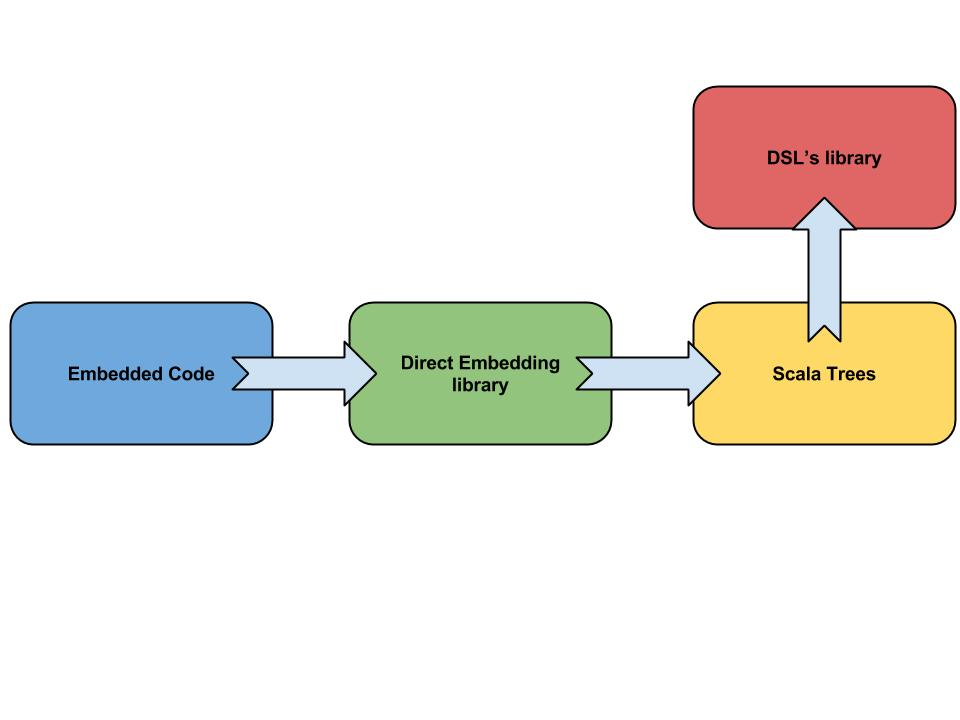
\includegraphics[width=0.8\linewidth]{./img/flow.jpg}
\end{figure}
\end{frame}

%------------------------------------------------
\subsection{Example}

\begin{frame}
\frametitle{An example: embedded code}
\begin{block}{Annotate}
@reifyAs(\TCM{\textbf{J}ustArgs})\\
\TCR{def} \TCB{justArgs}(x: Int): Int = ???
\end{block}

\begin{block}{Lift}
lift \{\\
~ ObjectExample.\TCB{justArgs}(1)\\
\}
\end{block}

\end{frame}

%------------------------------------------------

\begin{frame}
\frametitle{An example: tree}
\begin{block}{Tree}
ObjectExample.\TCB{justArgs}(1)\\
~ \textit{annotated}\\
directembedding.reifyAs(\TCM{\textbf{J}ustArgs})\\
\end{block}

\begin{block}{Raw tree}
Apply(Select(Ident(ch.epfl.directembedding.test.ObjectExample), TermName("justArgs")), List(Literal(Constant(1))))
\end{block}

\end{frame}

%------------------------------------------------

\begin{frame}
\frametitle{An example: macro}

From symbol, arguments, type, we can use the annotation to reify the tree:
\begin{block}{Macro}
 $\implies$ macro q"..."
\end{block}

\begin{block}{Returns}
\TCR{\textbf{J}}ustArgs.apply(1)
\end{block}

\end{frame}

%------------------------------------------------

\begin{frame}
\frametitle{Going further}

\begin{itemize}
\item ...
\end{itemize}

\end{frame}

%------------------------------------------------
\section{Demo}
\begin{frame}
\Huge{\centerline{Demo}}
\end{frame}

%------------------------------------------------

\begin{frame}
\Huge{\centerline{Thank you}}
\end{frame}

%------------------------------------------------

%\begin{frame}[fragile] % Need to use the fragile option when verbatim is used in the slide
%\frametitle{Citation}
%An example of the \verb|\cite| command to cite within the presentation:\\~
%
%This statement requires citation \cite{p1}.
%\end{frame}

%------------------------------------------------

%\begin{frame}
%\frametitle{References}
%\footnotesize{
%\begin{thebibliography}{99} % Beamer does not support BibTeX so references must be inserted manually as below
%\bibitem[Smith, 2012]{p1} John Smith (2012)
%\newblock Title of the publication
%\newblock \emph{Journal Name} 12(3), 45 -- 678.
%\end{thebibliography}
%}
%\end{frame}

%------------------------------------------------

%\begin{frame}[fragile] % Need to use the fragile option when verbatim is used in the slide
%\frametitle{Verbatim}
%\begin{block}{...}[Theorem Slide Code]
%\begin{verbatim}
%\begin{frame}
%\frametitle{Theorem}
%\begin{theorem}[Mass--energy equivalence]
%$E = mc^2$
%\end{theorem}
%\end{frame}\end{verbatim}
%\end{block}{...}
%\end{frame}

%----------------------------------------------------------------------------------------

\end{document} 